\documentclass[9pt]{beamer}

\beamertemplatenavigationsymbolsempty
\renewcommand\mathfamilydefault{cmr}

\usepackage{xcolor}
\usepackage{pajmath}
\usepackage{booktabs}
\usepackage{colortbl}
\usepackage{tikz}
\usetikzlibrary{calc}
\usetikzlibrary{intersections}
\usetikzlibrary{datavisualization}
\usetikzlibrary{datavisualization.formats.functions}

\title{Neural Networks: Perceptrons}
\date{Spring 2021}

\begin{document}

\maketitle

\begin{frame}{The artificial neuron}

A neuron connects a series on inputs (dendrites) to an output (axon).

\begin{center}
	output: $y$
	\raisebox{-0.2in}{\includegraphics[width=0.5\textwidth]{neuron}}
	$\left. \begin{matrix}x_1\\x_2\\ \vdots\\ x_n\end{matrix} \right\rbrace$ inputs
\end{center}
\pause
Our model needs to include two processes:
\begin{enumerate}
	\item The cell body (soma) combines all of the $n$ inputs.
	\item If the combined input exceeds a threshold, the output fires.
\end{enumerate}

\end{frame}

\begin{frame}{Modeling the artificial neuron}

\begin{center}
	output: $y$
	\raisebox{-0.2in}{\includegraphics[width=0.5\textwidth]{neuron}}
	$\left. \begin{matrix}x_1\\x_2\\ \vdots\\ x_n\end{matrix} \right\rbrace$ inputs
\end{center}
\bigskip
Let's model the combined input $z$ as a linear combination of the inputs.
\[ z = w_1x_1 + w_2x_2 + \cdots + w_nx_n = \V{w}\cdot\Vx \]

\pause
\bigskip
For now, let's assume the neuron ``fires'' based on the sign of $z$:
\[ y = \begin{cases} +1, & \V{w}\cdot\Vx > 0 \\ -1, & \V{w}\cdot\Vx < 0 \end{cases} \]

\end{frame}

\begin{frame}{Learning to classify}

Let's assume we have $n$ training points $(\Vx_i,y_i)$. How can we use these data to find the weights $\V{w}$ so the neuron fires only when $y_i=+1$?

\bigskip
\pause
\textbf{The Perceptron Update Algorithm}
\begin{enumerate}
	\item Choose a random vector of initial weights $\V{w}^{(0)}$ and a step size $\alpha$.
	\item For each training point $(\Vx_i,y_i)$, update the weights by
	\[ \V{w}^{(k+1)} = \begin{cases} \V{w}^{(k)} + \alpha y_i\Vx_i, & \text{if $\Vx_i$ is misclassified} \\ \V{w}^{(k)}, & \text{otherwise} \end{cases} \]
	\item Repeat until all points are classified correctly.
\end{enumerate}
	
\end{frame}

\begin{frame}{Does it work?}

\begin{columns}
\begin{column}{0.5\textwidth}
	\begin{center}
		\includegraphics[width=\textwidth]{HeartAttackSVM}
		
		Heart attack classification by SVM. \newline
	\end{center}
\end{column}

\begin{column}{0.5\textwidth}
	\begin{center}
		\includegraphics[width=\textwidth]{HeartAttackPerceptron}
		
		Heart attack classification by a perceptron.
	\end{center}
\end{column}
	
\end{columns}

\end{frame}

\begin{frame}{Why does it work?}

\begin{columns}

\begin{column}{0.33\textwidth}
\begin{center}
	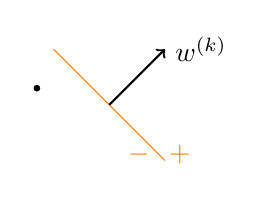
\begin{tikzpicture}
		\begin{scope}[rotate=-45]
			\draw [orange] (-1,0) -- (0.9,0) node [right] {$+$} node [left] {$-$} -- (1,0);
			\draw [black,thick,->] (0,0) -- (0,1) node [right] {$\V{w}^{(k)}$};
			\filldraw (-0.8,-0.5) circle (1pt) node [below] {$\Vx$};
		\end{scope}
	\end{tikzpicture}
	
	\bigskip
	Point \Vx\ is $+1$ and is therefore misclassified by $\V{w}^{(k)}$.
\end{center}
\end{column}

\pause
\begin{column}{0.33\textwidth}
\begin{center}
The weight is updated by
\[ \V{w}^{(k+1)} = \V{w}^{(k)} + \alpha\Vx, \]
tilting $\V{w}$ toward \Vx.
\end{center}
\end{column}

\pause
\begin{column}{0.33\textwidth}
\begin{center}
	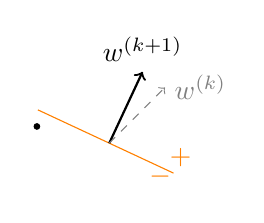
\begin{tikzpicture}
		\begin{scope}[rotate=-45]
			\begin{scope}[rotate=20]
				\draw [orange] (-1,0) -- (0.9,0) (1,0) node [above] {$+$} node [left] {$-$} -- (1,0);
				\draw [black,thick,->] (0,0) -- (0,1) node [above] {$\V{w}^{(k+1)}$};
			\end{scope}
			\draw [gray,dashed,->] (0,0) -- (0,1) node [right] {$\V{w}^{(k)}$};
			\filldraw (-0.8,-0.5) circle (1pt) node [below] {$\Vx$};
		\end{scope}
	\end{tikzpicture}
	
	\bigskip
	The new hyperplane is rotated toward \Vx\ so the point will eventually be on the correct side.
\end{center}
\end{column}

\end{columns}
\end{frame}

\begin{frame}{Wait, what happened to the intercept?}

The SVM problem used a linear classifier
\[ y = \begin{cases} +1, & \Va\cdot\Vx \ge b \\ -1, & \Va\cdot\Vx \le b \end{cases} \]
but our perceptron fires using the rule
\[ y = \begin{cases} +1, & \V{w}\cdot\Vx > 0 \\ -1, & \V{w}\cdot\Vx < 0 \end{cases} \]
Does this mean the perceptron hyperplane always passes through the origin?

\bigskip
\pause
\textbf{No.} We use a common ML trick to move the \emph{bias} (intercept) into the weight vector and expand \Vx\ with a dummy dimension containing 1.
\[ \V{w}\cdot\Vx = b \Leftrightarrow \vecthree{w_1}{w_2}{-b}\cdot\vecthree{x_1}{x_2}{1} = 0 \]

	
\end{frame}


\newcommand\hi{{$+1$}}
\newcommand\lo{{\color{red}$-1$}}
\newcommand\here{$\leftarrow$}


\begin{frame}{Example: Training a 2D Perceptron}
\begin{columns}
\begin{column}{0.6\textwidth}
	\begin{center}
		\begin{tabular}{rrrl}
			\toprule
			$x_1$ & $x_2$ & $y$ \\
			\cmidrule{1-3}
			$1$ & $0.9$ & \hi \\
		     $-1$ & $0.3$ & \hi \\
		     $0$ & $0.5$ & \hi \\
		     $1$ & $-1$ & \lo \\
		     $-0.5$ & $-0.7$ & \lo \\
		     $0.4$ & $-0.3$	& \lo \\
		    \bottomrule
		\end{tabular}

		\begin{align*}
			k &= 0,\quad\text{accuracy} = 4/6 \\
			\V{w}^{(0)} &= \transpose{(-0.2, 0.05, 0.03)} \\
		\end{align*}
	\end{center}
\end{column}

\begin{column}{0.4\textwidth}
	\begin{center}
	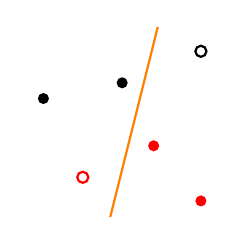
\begin{tikzpicture}
		\def\cz{2pt}
		\clip (-1.2,-1.2) rectangle (1.2,1.2);
		\draw [thick] (1,0.9) circle (\cz);
		\fill (-1,0.3) circle (\cz);
		\fill (0,0.5) circle (\cz);
		\fill [red] (1,-1) circle (\cz);
		\draw [thick,red] (-0.5,-0.7) circle (\cz);
		\fill [red] (0.4,-0.3) circle (\cz);
		\draw [orange,thick] (2,7.4) -- (-2,-8.6);
	\end{tikzpicture}
	\end{center}
\end{column}
\end{columns}
\end{frame}


% ========== 0-0 ============
\begin{frame}{Example: Training a 2D Perceptron}
\begin{columns}
\begin{column}{0.6\textwidth}
	\begin{center}
		\begin{tabular}{rrrl}
			\toprule
			$x_1$ & $x_2$ & $y$ \\
			\cmidrule{1-3}
			$1$ & $0.9$ & \hi & \here \\
		     $-1$ & $0.3$ & \hi \\
		     $0$ & $0.5$ & \hi \\
		     $1$ & $-1$ & \lo \\
		     $-0.5$ & $-0.7$ & \lo \\
		     $0.4$ & $-0.3$	& \lo \\
		    \bottomrule
		\end{tabular}

		\begin{align*}
			k &= 0,\quad\text{accuracy} = 4/6 \\
			\V{w}^{(0)} &= \transpose{(-0.2, 0.05, 0.03)} \\
			\V{w}^{(0)}\cdot\Vx &= -0.125\quad\text{(mismatch)} \\
			\V{w}^{(1)} &= \V{w}^{(0)} + 0.1(+1)\Vx \\
						&= \transpose{(-0.1, 0.14, 0.13)}
		\end{align*}
	\end{center}
\end{column}

\begin{column}{0.4\textwidth}
	\begin{center}
	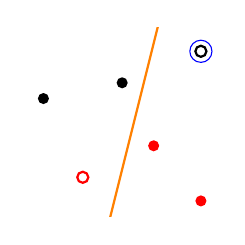
\begin{tikzpicture}
		\def\cz{2pt}
		\clip (-1.2,-1.2) rectangle (1.2,1.2);
		\draw [thick] (1,0.9) circle (\cz);
		\fill (-1,0.3) circle (\cz);
		\fill (0,0.5) circle (\cz);
		\fill [red] (1,-1) circle (\cz);
		\draw [thick,red] (-0.5,-0.7) circle (\cz);
		\fill [red] (0.4,-0.3) circle (\cz);
		\draw [orange,thick] (2,7.4) -- (-2,-8.6);
		\draw [blue] (1,0.9) circle (4pt);
	\end{tikzpicture}
	
	\pause
	\vspace{0.2in}
	\tikz{\draw[very thick,->] (0,1) -- (0,0);}
	\vspace{0.2in}
	
	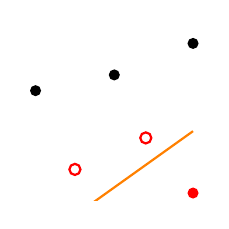
\begin{tikzpicture}
		\def\cz{2pt}
		\clip (-1.1,-1.1) rectangle (1.1,1.1);
		\fill (1,0.9) circle (\cz)
			  (-1,0.3) circle (\cz)
			  (0,0.5) circle (\cz);
		\fill [red]
			  (1,-1) circle (\cz);
		\draw [thick,red] (-0.5,-0.7) circle (\cz)
			  (0.4,-0.3) circle (\cz);
		\draw [orange,thick] (1,-0.214286) -- (-1,-1.64286);
	\end{tikzpicture}
	\end{center}
\end{column}
\end{columns}
\end{frame}

% ========== 1-1 ============
\begin{frame}{Example: Training a 2D Perceptron}
\begin{columns}
\begin{column}{0.6\textwidth}
	\begin{center}
		\begin{tabular}{rrrl}
			\toprule
			$x_1$ & $x_2$ & $y$ \\
			\cmidrule{1-3}
			$1$ & $0.9$ & \hi &  \\
		     $-1$ & $0.3$ & \hi & \here \\
		     $0$ & $0.5$ & \hi \\
		     $1$ & $-1$ & \lo \\
		     $-0.5$ & $-0.7$ & \lo \\
		     $0.4$ & $-0.3$	& \lo \\
		    \bottomrule
		\end{tabular}

		\begin{align*}
			k &= 1,\quad\text{accuracy} = 4/6 \\
			\V{w}^{(1)} &= \transpose{(-0.1, 0.14, 0.13)} \\
			\V{w}^{(1)}\cdot\Vx &= 0.272\quad\text{(match)} \\
			\V{w}^{(2)} &= \V{w}^{(1)}
		\end{align*}
	\end{center}
\end{column}

\begin{column}{0.4\textwidth}
	\begin{center}
	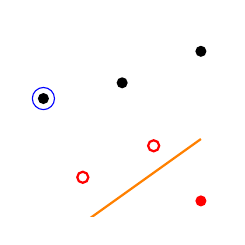
\begin{tikzpicture}
		\def\cz{2pt}
		\clip (-1.2,-1.2) rectangle (1.2,1.2);
		\fill (1,0.9) circle (\cz)
			  (-1,0.3) circle (\cz)
			  (0,0.5) circle (\cz);
		\fill [red]
			  (1,-1) circle (\cz);
		\draw [thick,red] (-0.5,-0.7) circle (\cz)
			  (0.4,-0.3) circle (\cz);
		\draw [orange,thick] (1,-0.214286) -- (-1,-1.64286);
		\draw [blue] (-1,0.3) circle (4pt);
	\end{tikzpicture}
	
	\pause
	\vspace{0.2in}
	\tikz{\draw[very thick,->] (0,1) -- (0,0);}
	\vspace{0.2in}
	
	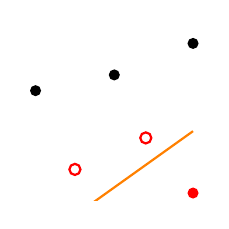
\begin{tikzpicture}
		\def\cz{2pt}
		\clip (-1.1,-1.1) rectangle (1.1,1.1);
		\fill (1,0.9) circle (\cz)
			  (-1,0.3) circle (\cz)
			  (0,0.5) circle (\cz);
		\fill [red]
			  (1,-1) circle (\cz);
		\draw [thick,red] (-0.5,-0.7) circle (\cz)
			  (0.4,-0.3) circle (\cz);
		\draw [orange,thick] (1,-0.214286) -- (-1,-1.64286);
	\end{tikzpicture}
	\end{center}
\end{column}
\end{columns}
\end{frame}

% ========== 1-2 ============
\begin{frame}{Example: Training a 2D Perceptron}
\begin{columns}
\begin{column}{0.6\textwidth}
	\begin{center}
		\begin{tabular}{rrrl}
			\toprule
			$x_1$ & $x_2$ & $y$ \\
			\cmidrule{1-3}
			$1$ & $0.9$ & \hi &  \\
		     $-1$ & $0.3$ & \hi &  \\
		     $0$ & $0.5$ & \hi & \here \\
		     $1$ & $-1$ & \lo \\
		     $-0.5$ & $-0.7$ & \lo \\
		     $0.4$ & $-0.3$	& \lo \\
		    \bottomrule
		\end{tabular}

		\begin{align*}
			k &= 2,\quad\text{accuracy} = 4/6 \\
			\V{w}^{(2)} &= \transpose{(-0.1, 0.14, 0.13)} \\
			\V{w}^{(2)}\cdot\Vx &= 0.2\quad\text{(match)} \\
			\V{w}^{(3)} &= \V{w}^{(2)}
		\end{align*}
	\end{center}
\end{column}

\begin{column}{0.4\textwidth}
	\begin{center}
	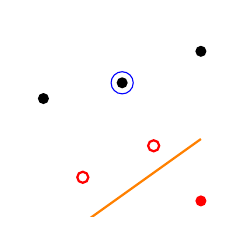
\begin{tikzpicture}
		\def\cz{2pt}
		\clip (-1.2,-1.2) rectangle (1.2,1.2);
		\fill (1,0.9) circle (\cz)
			  (-1,0.3) circle (\cz)
			  (0,0.5) circle (\cz);
		\fill [red]
			  (1,-1) circle (\cz);
		\draw [thick,red] (-0.5,-0.7) circle (\cz)
			  (0.4,-0.3) circle (\cz);
		\draw [orange,thick] (1,-0.214286) -- (-1,-1.64286);
		\draw [blue] (0,0.5) circle (4pt);
	\end{tikzpicture}
	
	\pause
	\vspace{0.2in}
	\tikz{\draw[very thick,->] (0,1) -- (0,0);}
	\vspace{0.2in}
	
	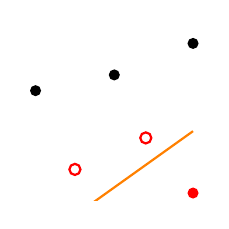
\begin{tikzpicture}
		\def\cz{2pt}
		\clip (-1.1,-1.1) rectangle (1.1,1.1);
		\fill (1,0.9) circle (\cz)
			  (-1,0.3) circle (\cz)
			  (0,0.5) circle (\cz);
		\fill [red]
			  (1,-1) circle (\cz);
		\draw [thick,red] (-0.5,-0.7) circle (\cz)
			  (0.4,-0.3) circle (\cz);
		\draw [orange,thick] (1,-0.214286) -- (-1,-1.64286);
	\end{tikzpicture}
	\end{center}
\end{column}
\end{columns}
\end{frame}

% ========== 1-3 ============
\begin{frame}{Example: Training a 2D Perceptron}
\begin{columns}
\begin{column}{0.6\textwidth}
	\begin{center}
		\begin{tabular}{rrrl}
			\toprule
			$x_1$ & $x_2$ & $y$ \\
			\cmidrule{1-3}
			$1$ & $0.9$ & \hi &  \\
		     $-1$ & $0.3$ & \hi &  \\
		     $0$ & $0.5$ & \hi &  \\
		     $1$ & $-1$ & \lo & \here \\
		     $-0.5$ & $-0.7$ & \lo \\
		     $0.4$ & $-0.3$	& \lo \\
		    \bottomrule
		\end{tabular}

		\begin{align*}
			k &= 3,\quad\text{accuracy} = 4/6 \\
			\V{w}^{(3)} &= \transpose{(-0.1, 0.14, 0.13)} \\
			\V{w}^{(3)}\cdot\Vx &= -0.11\quad\text{(match)} \\
			\V{w}^{(4)} &= \V{w}^{(3)}
		\end{align*}
	\end{center}
\end{column}

\begin{column}{0.4\textwidth}
	\begin{center}
	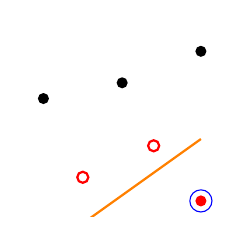
\begin{tikzpicture}
		\def\cz{2pt}
		\clip (-1.2,-1.2) rectangle (1.2,1.2);
		\fill (1,0.9) circle (\cz)
			  (-1,0.3) circle (\cz)
			  (0,0.5) circle (\cz);
		\fill [red]
			  (1,-1) circle (\cz);
		\draw [thick,red] (-0.5,-0.7) circle (\cz)
			  (0.4,-0.3) circle (\cz);
		\draw [orange,thick] (1,-0.214286) -- (-1,-1.64286);
		\draw [blue] (1,-1) circle (4pt);
	\end{tikzpicture}
	
	\pause
	\vspace{0.2in}
	\tikz{\draw[very thick,->] (0,1) -- (0,0);}
	\vspace{0.2in}
	
	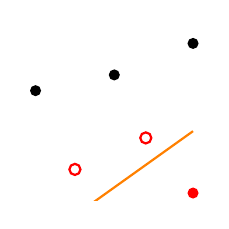
\begin{tikzpicture}
		\def\cz{2pt}
		\clip (-1.1,-1.1) rectangle (1.1,1.1);
		\fill (1,0.9) circle (\cz)
			  (-1,0.3) circle (\cz)
			  (0,0.5) circle (\cz);
		\fill [red]
			  (1,-1) circle (\cz);
		\draw [thick,red] (-0.5,-0.7) circle (\cz)
			  (0.4,-0.3) circle (\cz);
		\draw [orange,thick] (1,-0.214286) -- (-1,-1.64286);
	\end{tikzpicture}
	\end{center}
\end{column}
\end{columns}
\end{frame}

% ========== 1-4 ============
\begin{frame}{Example: Training a 2D Perceptron}
\begin{columns}
\begin{column}{0.6\textwidth}
	\begin{center}
		\begin{tabular}{rrrl}
			\toprule
			$x_1$ & $x_2$ & $y$ \\
			\cmidrule{1-3}
			$1$ & $0.9$ & \hi &  \\
		     $-1$ & $0.3$ & \hi &  \\
		     $0$ & $0.5$ & \hi &  \\
		     $1$ & $-1$ & \lo & \\
		     $-0.5$ & $-0.7$ & \lo & \here \\
		     $0.4$ & $-0.3$	& \lo \\
		    \bottomrule
		\end{tabular}

		\begin{align*}
			k &= 4,\quad\text{accuracy} = 4/6 \\
			\V{w}^{(4)} &= \transpose{(-0.1, 0.14, 0.13)} \\
			\V{w}^{(4)}\cdot\Vx &= 0.082\quad\text{(mismatch)} \\
			\V{w}^{(5)} &= \V{w}^{(4)} + 0.1(-1)\Vx \\
						&= \transpose{(-0.05, 0.21, 0.03)}
		\end{align*}
	\end{center}
\end{column}

\begin{column}{0.4\textwidth}
	\begin{center}
	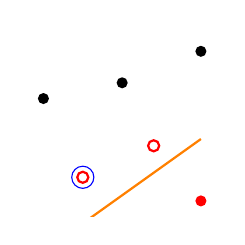
\begin{tikzpicture}
		\def\cz{2pt}
		\clip (-1.2,-1.2) rectangle (1.2,1.2);
		\fill (1,0.9) circle (\cz)
			  (-1,0.3) circle (\cz)
			  (0,0.5) circle (\cz);
		\fill [red]
			  (1,-1) circle (\cz);
		\draw [thick,red] (-0.5,-0.7) circle (\cz)
			  (0.4,-0.3) circle (\cz);
		\draw [orange,thick] (1,-0.214286) -- (-1,-1.64286);
		\draw [blue] (-0.5,-0.7) circle (4pt);
	\end{tikzpicture}
	
	\pause
	\vspace{0.2in}
	\tikz{\draw[very thick,->] (0,1) -- (0,0);}
	\vspace{0.2in}
	
	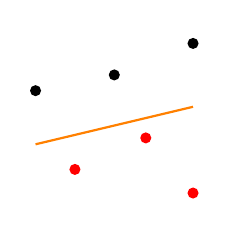
\begin{tikzpicture}
		\def\cz{2pt}
		\clip (-1.1,-1.1) rectangle (1.1,1.1);
		\fill (1,0.9) circle (\cz)
			  (-1,0.3) circle (\cz)
			  (0,0.5) circle (\cz);
		\fill [red]
			  (1,-1) circle (\cz)
			  (-0.5,-0.7) circle (\cz)
			  (0.4,-0.3) circle (\cz);
		\draw [orange,thick] (1,0.0952381) -- (-1,-0.380952);
	\end{tikzpicture}
	\end{center}
\end{column}
\end{columns}
\end{frame}

% ========== 1-5 ============
\begin{frame}{Example: Training a 2D Perceptron}
\begin{columns}
\begin{column}{0.6\textwidth}
	\begin{center}
		\begin{tabular}{rrrl}
			\toprule
			$x_1$ & $x_2$ & $y$ \\
			\cmidrule{1-3}
			$1$ & $0.9$ & \hi &  \\
		     $-1$ & $0.3$ & \hi &  \\
		     $0$ & $0.5$ & \hi &  \\
		     $1$ & $-1$ & \lo & \\
		     $-0.5$ & $-0.7$ & \lo & \\
		     $0.4$ & $-0.3$	& \lo & \here \\
		    \bottomrule
		\end{tabular}

		\begin{align*}
			k &= 5,\quad\text{accuracy} = 6/6 \\
			\V{w}^{(5)} &= \transpose{(-0.05, 0.21, 0.03)} \\
			\V{w}^{(5)}\cdot\Vx &= -0.05\quad\text{(match)} \\
			\V{w}^{(6)} &= \V{w}^{(5)}
		\end{align*}
	\end{center}
\end{column}

\begin{column}{0.4\textwidth}
	\begin{center}
	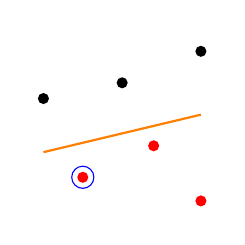
\begin{tikzpicture}
		\def\cz{2pt}
		\clip (-1.2,-1.2) rectangle (1.2,1.2);
		\fill (1,0.9) circle (\cz)
			  (-1,0.3) circle (\cz)
			  (0,0.5) circle (\cz);
		\fill [red]
			  (1,-1) circle (\cz)
			  (-0.5,-0.7) circle (\cz)
			  (0.4,-0.3) circle (\cz);
		\draw [orange,thick] (1,0.0952381) -- (-1,-0.380952);
		\draw [blue] (-0.5,-0.7) circle (4pt);
	\end{tikzpicture}
	
	\pause
	\vspace{0.2in}
	\tikz{\draw[very thick,->] (0,1) -- (0,0);}
	\vspace{0.2in}
	
	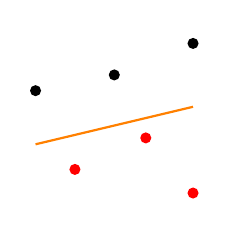
\begin{tikzpicture}
		\def\cz{2pt}
		\clip (-1.1,-1.1) rectangle (1.1,1.1);
		\fill (1,0.9) circle (\cz)
			  (-1,0.3) circle (\cz)
			  (0,0.5) circle (\cz);
		\fill [red]
			  (1,-1) circle (\cz)
			  (-0.5,-0.7) circle (\cz)
			  (0.4,-0.3) circle (\cz);
		\draw [orange,thick] (1,0.0952381) -- (-1,-0.380952);
	\end{tikzpicture}
	\end{center}
\end{column}
\end{columns}
\end{frame}

\begin{frame}{Summary}

\begin{itemize}
	\item A perceptron is a simplistic model of a single neuron.
	\item A perceptron can learn to perform simple classification tasks using an update rule.
	\item<2-> \textbf{Next time:} Imagine what a network of millions of perceptrons can learn!
\end{itemize}
	
\end{frame}


\end{document}
